%%%%%%%%%%%%%%%%%%%%%%%%%%%%%%%%%%%%%%%%%%%%%%%%%%%%%%%%%%%%%%%%%%%%%%%%%%%%%%%%
%                       EXPERIMENT DATASETS CHES                               %
%%%%%%%%%%%%%%%%%%%%%%%%%%%%%%%%%%%%%%%%%%%%%%%%%%%%%%%%%%%%%%%%%%%%%%%%%%%%%%%%
So far, we have considered our experimental investigations through the view of the Leakage Assessment Problem (\ie{} \autoref{leak_assess}).
However, we remind that the final task an evaluator is given to achieve is the profiled \gls{sca} optimization (\ie{} \autoref{final_task_prof}), namely to find \(\numTracesAttackOpt\).

It is recalled that \autoref{cor:main_result} argued that by solving the Leakage Assessment Problem, one could get an accurate estimation \(\numTracesAttackEst{\MLmodelMLE{\trainSet}}\) of the quantity \(\frac{f(\beta)}{\MI{\Z}{\XXX}}\), known to be a lower-bound of the optimal solution of the profiled \gls{sca} optimization problem, namely \(\numTracesAttackOpt\).

One could wonder whether this inequality still holds for any model, maybe sub-optimal, \ie{} when estimating the minimal number of queries \(\numTracesAttack(\MLmodel)\) to the target device for such a model with the quantity \(\numTracesAttackEst{\MLmodel}\).
A formal proof would be a promising further work, though beyond the scope of this thesis.%
\footnote{
    We discuss in \autoref{sec:ccl_ches} the recent improvements proposed following this work.
}
Nevertheless we propose here to empirically verify this hypothesis by training a \gls{cnn} on all the public datasets presented in \autoref{sec:datasets} and by implementing the key enumeration in order to evaluate \(\numTracesAttack(\MLmodel)\).%
\footnote{
    See the method described in \autoref{sec:estimate_practice} for the practical estimation of \(\numTracesAttack(\MLmodel)\).
}
This way, our claim can be tested under several cases covering all the counter-measures considered in this thesis.

\paragraph{Settings.}
For each training, a \gls{vgg}-like \gls{cnn} architecture has been used, as presented in \autoref{sec:pres_architectures}.
More specifically:
\begin{itemize}
    \item \textbf{\gls{ascad} and \gls{aeshd}}:
    the following parameters have been used: \(n_1 = 2\), \(n_2 = 7\), the convolutional filters are of length \(\ksize=11\) and the pooling stride is \(\pstride=2\).
    \(\numFilters = 10\) filters are in the first layer, and they are doubled at each convolutional layer.
    The last pooling layer has a stride set so that the output size along the time dimensionality is one.
    The dense layers contains \(1,000\) intermediate neurons.
    This architecture is based on our works presented at \textsc{Cosade}'19 and is more thoroughly discussed in \autoref{sec:with_mask_no_desynchro}
    \item \textbf{\gls{aesrd}}: the same \gls{vgg}-like architecture as the one presented by Kim \etal{}~\cite{kim_make_2019} has been used.
    More specifically, \(n_2\) is set to \(9\) so that there is enough pooling layers to get feature maps on the last convolutional layer whose width equals one.
    Besides, \(n_1=0\), \ie{} there is no intermediate dense layer, except softmax.
    \item \textbf{Polymorphism}: the precise architecture used for the experiments is the one used in our works presented at \textsc{Esorics}'20 and a whole dedicated discussion is proposed in \autoref{sec:cnn_archi_esorics}.
\end{itemize}

The training has been run on \(200\) epochs on the \gls{aesrd} and the Polymorphism datasets, \(50\) epochs on the \gls{aeshd} dataset, and stopped after \(30\) epochs on the \gls{ascad} dataset -- see an explanation in \autoref{sec:with_mask_no_desynchro}.
After each epoch \(t\) the optimization algorithm -- \gls{adam} here -- returns an update of the learning parameter vector denoted by \(\MLparam_t\).
We can therefore estimate the efficiency of the -- partially optimized -- model \(\MLmodel(\cdot, \MLparam_t)\), \ie{} \(\numTracesAttack\left(\MLmodel(\cdot, \MLparam_t)\right)\) thanks to a key enumeration, according to the procedure detailed in \autoref{sec:estimate_practice}.

\begin{figure}
    \centering
    \begin{subfigure}{0.49\textwidth}
        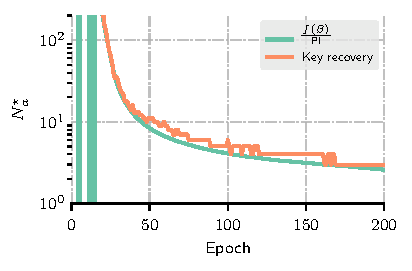
\includegraphics{Figures/experiments/RD_demo}
        \caption{\gls{aesrd} dataset.}
        \label{fig:ches_aes_rd}
    \end{subfigure}
    \begin{subfigure}{0.49\textwidth}
        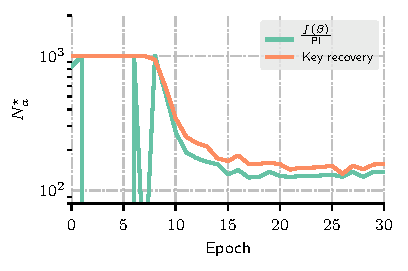
\includegraphics{Figures/experiments/ASCAD_demo}
        \caption{\gls{ascad} dataset}
        \label{fig:ches_ascad}
    \end{subfigure}
    \begin{subfigure}{0.49\textwidth}
        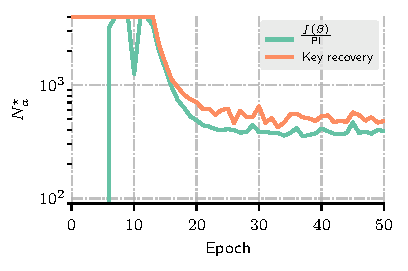
\includegraphics{Figures/experiments/AES_HD_demo}
        \caption{\gls{aeshd} dataset}
        \label{fig:ches_aes_hd}
    \end{subfigure}
    \begin{subfigure}{0.49\textwidth}
        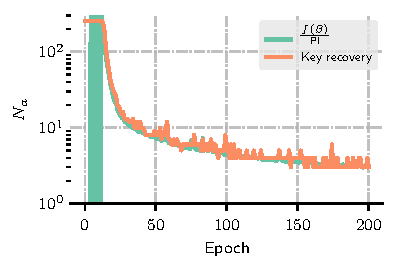
\includegraphics{Figures/experiments/mbedTLS}
        \caption{Polymorphism dataset (\mbedTLS{})}
        \label{fig:ches_mbedTLS}
    \end{subfigure}
    \begin{subfigure}{0.49\textwidth}
        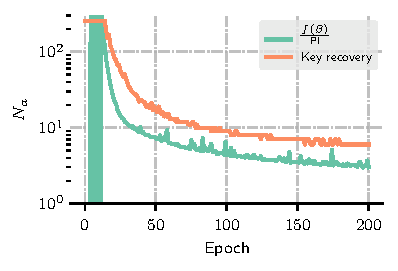
\includegraphics{Figures/experiments/aes_8bit_05}
        \caption{Polymorphism dataset (\aeshuitbit{})}
        \label{fig:ches_aes_8bit}
    \end{subfigure}
    \caption{Comparison between the estimation of \(\numTracesAttack(\MLmodel(\cdot, \MLparam_t))\) through the lower bound (orange lines) and through a key enumeration (green lines).}
    \label{fig:exp_pub_datasets}
\end{figure}

\paragraph{Results.}
The results are given in \autoref{fig:exp_pub_datasets}.
On each graph, \(\numTracesAttackEst{\MLmodel(\cdot, \MLparam_t)}\) is denoted in green, whereas the enumeration key estimation \(\numTracesAttack(\MLmodel(\cdot, \MLparam_t))\) is denoted by the orange curve.
Each curve has been clipped in order to be in \([0, 10^3]\), except for the \gls{aeshd} dataset where the high threshold is \(4.10^3\) since the literature presumed a higher \(\numTracesAttackOpt\)~\cite{kim_make_2019,zaid_methodology_2019}.


On \autoref{fig:ches_aes_rd}, we can remark that the first epochs of the profiling of the \gls{aesrd} dataset show a chaotic behavior.
This is explained by the fact that the \gls{nll} loss is initially close to \(n=8\) bits, or in other words, the \gls{pi} is close to zero, leading to unstable estimations of \(\numTracesAttackEst{\MLmodel(\cdot, \MLparam_t)}\). 
Once the model has started extracting some information, \ie{} after approximately epochs, the \gls{pi} starts to be significantly higher than \(0\) and the unstability vanishes. 
We can then observe that \(\numTracesAttackEst{\MLmodel(\cdot, \MLparam_t)}\) is always lower than the key enumeration estimation \(\numTracesAttack(\MLmodel(\cdot, \MLparam_t))\) as expected, while remaining tight through the epochs: the average relative error, computed starting the \(t=20\)-th epoch is of \(16\%\).
The final model is able to recover the secret key in \(3\) traces, and has a \gls{pi} of \(2.95\) bits/trace.%
\footnote{
    Those results coincide with the ones reported by Kim \etal{}~\cite{kim_make_2019}.
}

Likewise, for the \gls{ascad} dataset, the results are presented in \autoref{fig:ches_ascad}.
We can observe the same unstability at the beginning of the training, though the quantity \(\numTracesAttackEst{\MLmodel(\cdot, \MLparam_t)}\) remains lower than the estimation through the enumeration key afterwards, while staying quite tight.
The average relative error is also here of \(16\%\), and the final \gls{pi} is \(0.065\) bit/trace.

In addition, for the \gls{aeshd}, the results are presented in \autoref{fig:ches_aes_hd}.
Similarly to the two preceding experiments, a tight estimation is obtained, since the relative error is \(18\%\), while the final \gls{pi} is \(0.020\) bit/trace.

Finally, the outcomes on the two Polymorphism datasets are presented.
\autoref{fig:ches_mbedTLS} deals with the \mbedTLS{} implementation and depicts two superposed curves, hence a tight estimation of \(\numTracesAttack(\MLmodel(\cdot, \MLparam_t))\).
Similarly, \autoref{fig:ches_aes_8bit} deals with the \aeshuitbit{} implementation.
Although the estimation seems looser, the relative error remains of \(15\%\).

As a consequence, all those experiments tend to confirm that the quantities \(\numTracesAttackEst{\MLmodel(\cdot, \MLparam_t)}\) and \(\numTracesAttack(\MLmodel(\cdot, \MLparam_t))\) are effectively related, at least for a threshold \(\beta = 90\%\).
This is of great interest in the evaluation of the security of a device, since this not only empirically shows the relevance of minimizing the \gls{nll} loss, but this also provides a relevant tool to predict the required number of queries to succeed the key recovery, or at least to give a lower-bound to such a number, which is still useful since we look for a worst case scenario in a \gls{sca} evaluation.